\documentclass{article}

% Language setting
\usepackage[english]{babel}

% Set page size and margins
% Replace `letterpaper' with `a4paper' for UK/EU standard size
\usepackage[letterpaper,top=2cm,bottom=2cm,left=3cm,right=3cm,marginparwidth=1.75cm]{geometry}

% Useful packages
\usepackage{amsmath}
% --- Code listings ---
\usepackage{listings}
\usepackage{xcolor}
\definecolor{codegreen}{rgb}{0,0.6,0}
\definecolor{codegray}{rgb}{0.5,0.5,0.5}
\definecolor{codepurple}{rgb}{0.58,0,0.82}
\definecolor{backcolour}{rgb}{0.95,0.95,0.92}

\lstdefinestyle{mystyle}{
    backgroundcolor=\color{backcolour},   
    commentstyle=\color{codegreen},
    keywordstyle=\color{magenta},
    numberstyle=\tiny\color{codegray},
    stringstyle=\color{codepurple},
    basicstyle=\ttfamily\footnotesize,
    breakatwhitespace=false,         
    breaklines=true,                 
    captionpos=b,                    
    keepspaces=true,                 
    numbers=left,                    
    numbersep=5pt,                  
    showspaces=false,                
    showstringspaces=false,
    showtabs=false,                  
    tabsize=2
}

\lstset{style=mystyle}
% --- End Code Listings
\usepackage{graphicx}
\usepackage{float}
% \usepackage{caption}
% \usepackage{subcaption}
\usepackage[colorlinks=true, allcolors=blue]{hyperref}
\graphicspath{{./figures/}}

\title{ECE 637 - Lab 1}
\author{Colin Braun}

\begin{document}
\maketitle

\section{Section 3 Report - FIR Low Pass Filter}
\subsection{Derivation of analytical expression for $H(e^{ju}, e^{jv})$}
% TODO: Put this in
\subsection{Plot of $|H(e^{ju}, e^{jv})|$}
\begin{figure}[H]
    \centering
    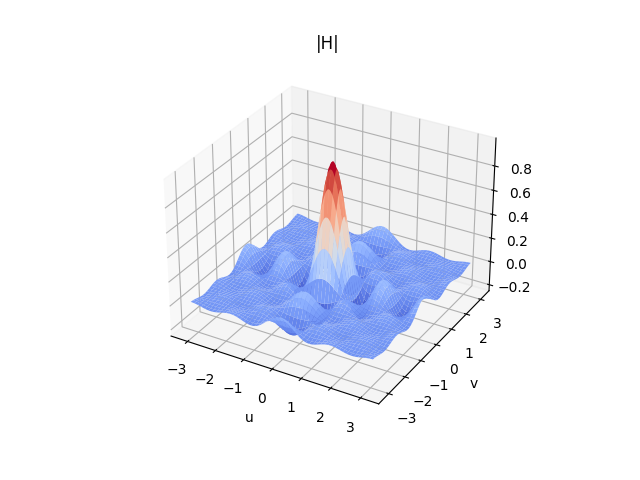
\includegraphics[width=0.75\textwidth]{../results/section3-python.png}
    \begin{center}
    %Figure 1(a): The frequency response of $H_m(\omega), m = 0,1,...,7$.
    \end{center}
    \label{fig:A1}
\end{figure}
\subsection{Color Image in img03.tif}
\begin{figure}[H]
    \centering
    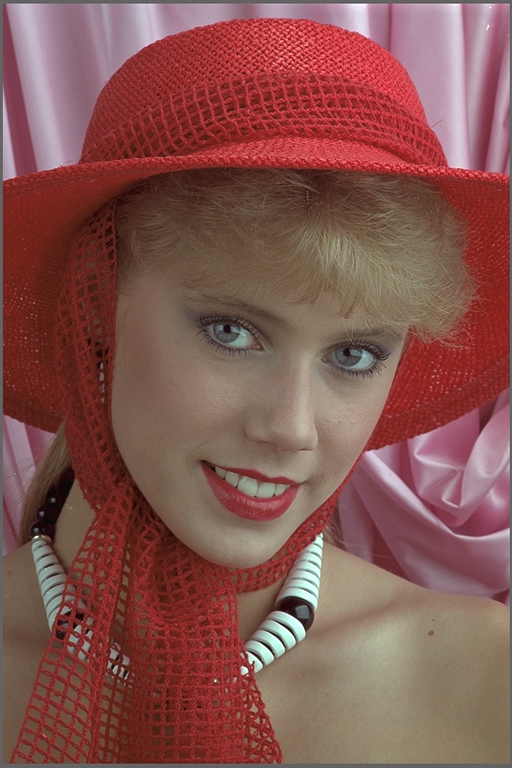
\includegraphics[width=0.75\textwidth]{../results/img03.png}
    \begin{center}
    %Figure 1(a): The frequency response of $H_m(\omega), m = 0,1,...,7$.
    \end{center}
    \label{fig:A1}
\end{figure}
\subsection{Filtered Color Image}
\begin{figure}[H]
    \centering
    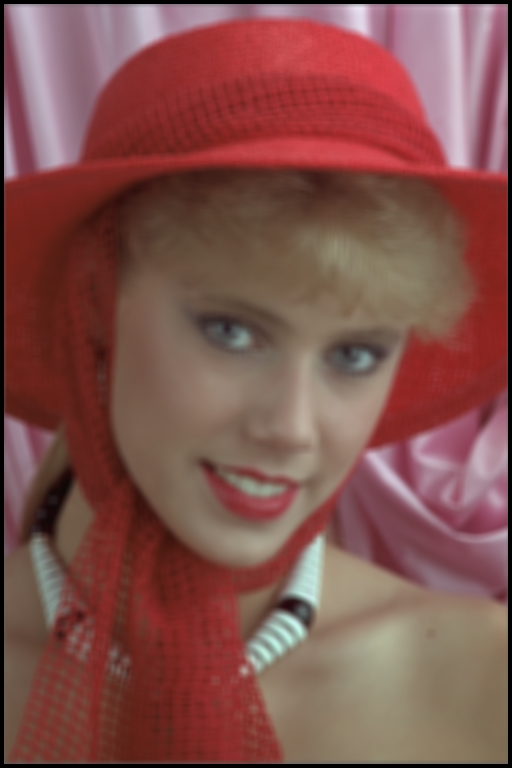
\includegraphics[width=0.75\textwidth]{../results/smoothed.png}
    \begin{center}
    %Figure 1(a): The frequency response of $H_m(\omega), m = 0,1,...,7$.
    \end{center}
    \label{fig:A1}
\end{figure}
\subsection{C Code}
The code used to generate this image.
\lstinputlisting[language=C]{../section3.c}

\section{Section 4 Report - FIR Sharpening Filter}
\subsection{Derivation of analytical expression for $H(e^{ju}, e^{jv})$}
% TODO: Put this in
\subsection{Derivation of analytical expression for $G(e^{ju}, e^{jv})$}
% TODO: Put this in
\subsection{Plot of $|H(e^{ju}, e^{jv})|$}
% TODO: Put this in
\begin{figure}[H]
    \centering
    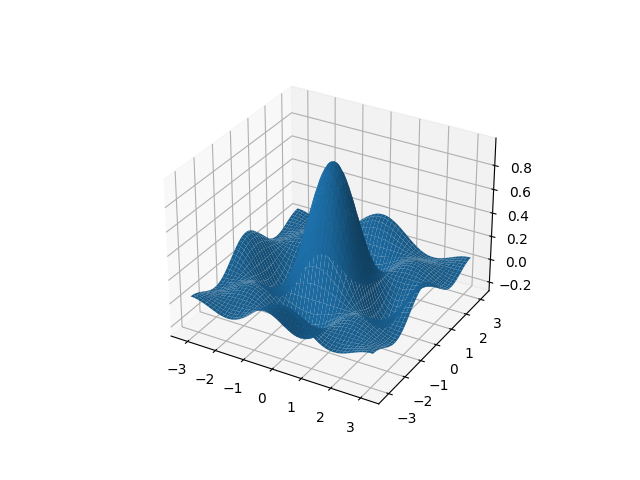
\includegraphics[width=0.75\textwidth]{../results/section4-H-python.png}
    \begin{center}
    %Figure 1(a): The frequency response of $H_m(\omega), m = 0,1,...,7$.
    \end{center}
    \label{fig:A1}
\end{figure}
\subsection{Plot of $|G(e^{ju}, e^{jv})|$ for $\lambda = 1.5$}
% TODO: Put this in
\begin{figure}[H]
    \centering
    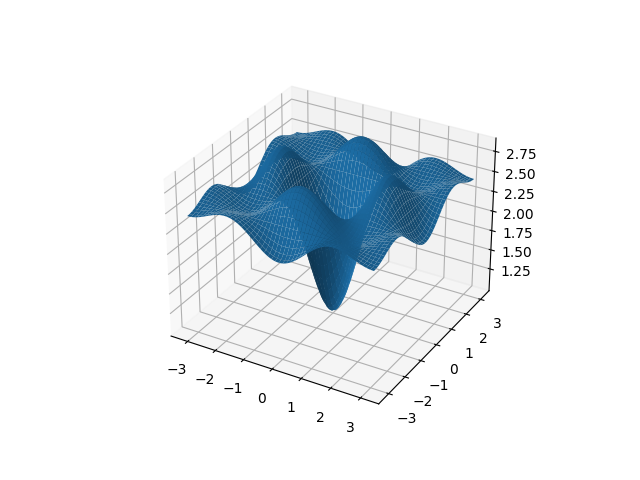
\includegraphics[width=0.75\textwidth]{../results/section4-G-python.png}
    \begin{center}
    %Figure 1(a): The frequency response of $H_m(\omega), m = 0,1,...,7$.
    \end{center}
    \label{fig:A1}
\end{figure}
\subsection{Input Color Image imgblur.tif}
\begin{figure}[H]
    \centering
    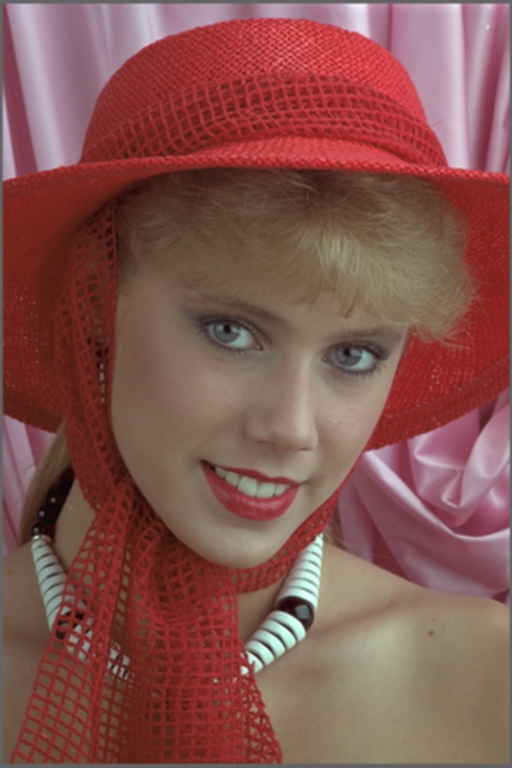
\includegraphics[width=0.75\textwidth]{../results/imgblur.png}
    \begin{center}
    %Figure 1(a): The frequency response of $H_m(\omega), m = 0,1,...,7$.
    \end{center}
    \label{fig:A1}
\end{figure}
\subsection{Sharpened Color Image for $\lambda = 1.5$}
\begin{figure}[H]
    \centering
    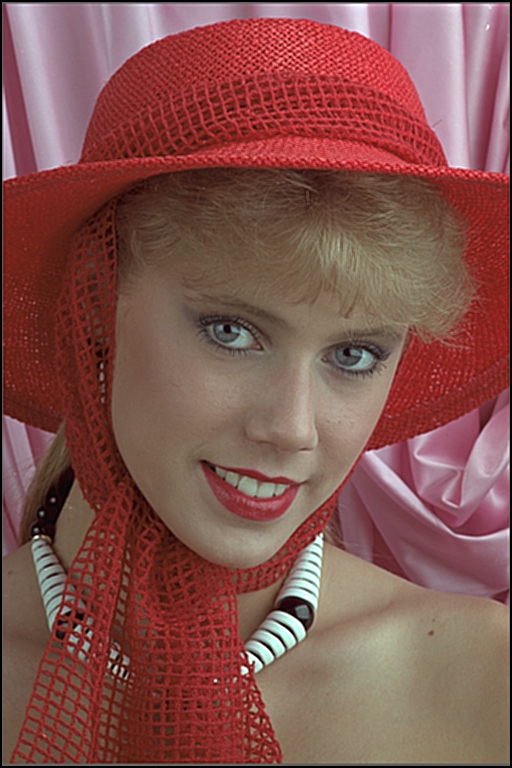
\includegraphics[width=0.75\textwidth]{../results/sharpened.png}
    \begin{center}
    %Figure 1(a): The frequency response of $H_m(\omega), m = 0,1,...,7$.
    \end{center}
    \label{fig:A1}
\end{figure}
\subsection{C Code}
%TODO: Put this in
\lstinputlisting[language=C]{../section4.c}

\section{Section 5 Report - IIR Filter}
\subsection{Derivation of analytical expression for $H(e^{ju}, e^{jv})$}
% TODO: Put this in
\subsection{Plot of $|H(e^{ju}, e^{jv})|$}
\begin{figure}[H]
    \centering
    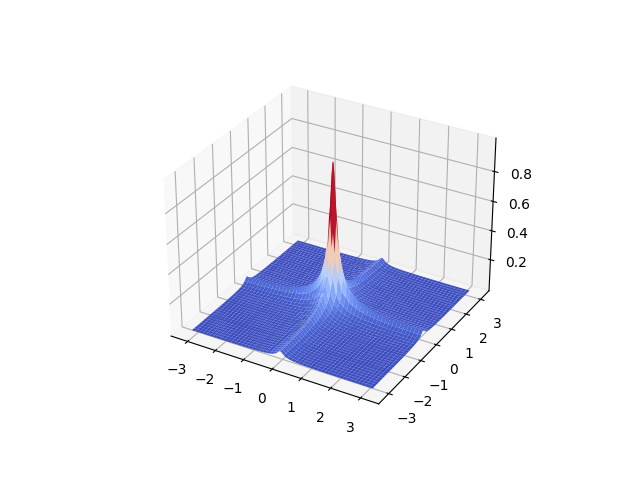
\includegraphics[width=0.75\textwidth]{../results/section5-python.png}
    \begin{center}
    %Figure 1(a): The frequency response of $H_m(\omega), m = 0,1,...,7$.
    \end{center}
    \label{fig:A1}
\end{figure}
\subsection{Image of Point Spread Function}
\begin{figure}[H]
    \centering
    
\includegraphics[width=0.75\textwidth]{../results/h_out.png}
    \begin{center}
    %Figure 1(a): The frequency response of $H_m(\omega), m = 0,1,...,7$.
    \end{center}
    \label{fig:A1}
\end{figure}
\subsection{Filtered Ouput Color Image}
%TODO: Put this in
\subsection{C Code}
\lstinputlisting[language=C]{../section5.c}
\begin{equation*}
    h_0[n] = h_{0}^{(2)}[n] \ast h_{0_2}^{(2)}[n] \ast h_{0_4}^{(2)}[n] \iff H_0(\omega) = H_0^{(2)}(\omega)H_0^{(2)}(2\omega)H_0^{(2)}(4\omega).
\end{equation*}

\section{Section 2}
First paragraph of section 2. Example Figure:
\begin{figure}[H]
    \centering
    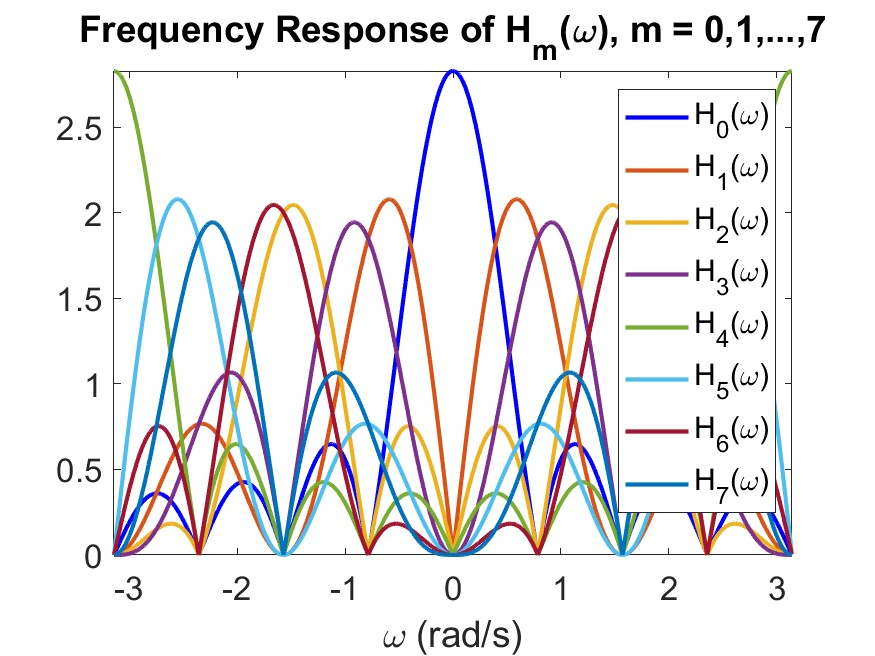
\includegraphics[width=0.75\textwidth]{figure-example}
    \begin{center}
    Figure 1(a): The frequency response of $H_m(\omega), m = 0,1,...,7$.
    \end{center}
    \label{fig:A1}
\end{figure}

Example Table
\begin{table}[H]
    \begin{center}
        \begin{tabular}{| l | l | l | l | l | l | l | l |}
            \hline
            1.0000 & 0 & 0 & 0 & 0 & 0 & 0 & 0 \\
            \hline
            0 & 1.0000 & 0 & 0 & 0 & 0 & 0 & 0 \\
            \hline
            0 & 0 & 1.0000 & 0 & 0 & 0 & 0 & 0 \\
            \hline
            0 & 0 & 0 & 1.0000 & 0 & 0 & 0 & 0 \\
            \hline
            0 & 0 & 0 & 0 & 1.0000 & 0 & 0 & 0 \\
            \hline
            0 & 0 & 0 & 0 & 0 & 1.0000 & 0 & 0 \\
            \hline
            0 & 0 & 0 & 0 & 0 & 0 & 1.0000 & 0 \\
            \hline
            0 & 0 & 0 & 0 & 0 & 0 & 0 & 1.0000 \\
            \hline
        \end{tabular}
    \end{center}
    \caption{$\textbf{HH}^{\dagger}$ is nearly identical to the identity matrix $\textbf{I}$.}
\end{table}

\section{Section 3}
Example of how to include code is below:
\lstinputlisting[language=Matlab]{code/example.m}

\end{document}
